%% ----------------------------------------------------------------
%% Chapter 6 -- Results and Discussion
%% ----------------------------------------------------------------
\chapter{Results and Discussion}
\label{chap:results}

Both fusion algorithms were simulated and then implemented on the dual core platform.

\section{DCI Performance During Line-of-Sight and Occlusion}
\label{sec:dci_results}

During line-of-sight conditions, the nominal standard deviation of the position estimates of the two sensors are 0.2~m$^2$ for radar and 2.0~m$^2$ for Wi-Fi. The value of omega, which represents the relative weights assigned to each sensor, can be computed using Equation~\ref{eq:omega_results}:

\begin{equation}
\omega = \frac{1/\sigma_{radar}^2}{1/\sigma_{radar}^2 + 1/P_{wifi}(t)}
\label{eq:omega_results}
\end{equation}

With nominal values inserted into the above equation, the resulting $\omega = 0.909$ or approximately 91\% weighting towards radar. As previously described, once line-of-sight is lost to the radar stream, both standard filters are subject to ``freshness blindness'' in which they lock onto the last received Wi-Fi measurement and produce stair-step type artifacts in their trajectory estimate. In contrast, the DCI algorithm prevents this by introducing an age of information penalty where the covariance of Wi-Fi increases linearly with time while a velocity model continues to provide good trajectory extrapolations. Stress test Results show raw radar MSE during occlusion is 17.93. Fused MSE is 9.86 representing a 45\% improvement.

\section{ML Fusion Accuracy}
\label{sec:ml_results}

A total of approximately 35,000 spatial events were reshaped as five-timestep rolling windows in order to train the neural network. Sensor missing values are filled by applying an early fill method, using binary freshness flags in order to prevent teleportation errors caused by filling missing values with zeros. Early stoppage was implemented during the training phase in order to avoid overfitting. Normalized mean squared errors (MSE) were calculated for each of the data split sets. These MSEs indicated that the normalized MSE for the training data was 0.000588, for the validation data was 0.000621, and for the testing data was 0.001958. The average absolute deviation (MAE) of the test-set range was found to be 0.118 meters; while the angular MAE was determined to be 4.88 degrees. The Euclidean P95 error was determined to be 0.555 meters.

\begin{table}[htbp]
\centering
\caption{Model accuracy metrics}
\label{tab:model_accuracy}
\begin{tabular}{lccc}
\toprule
\textbf{Metric} & \textbf{Train} & \textbf{Val} & \textbf{Test} \\
\midrule
MSE (norm)       & 0.000588       & 0.000621     & 0.001958      \\
MAE range (m)    & 0.107          & 0.078        & \textbf{0.118} \\
MAE angle ($^\circ$) & 2.09           & 3.02         & \textbf{4.88}  \\
Euclid. mean (m) & 0.168          & 0.144        & \textbf{0.256} \\
Euclid. 95th\% (m)& 0.385          & 0.276        & \textbf{0.555} \\
\bottomrule
\end{tabular}
\end{table}

\begin{figure}[htbp]
\centering
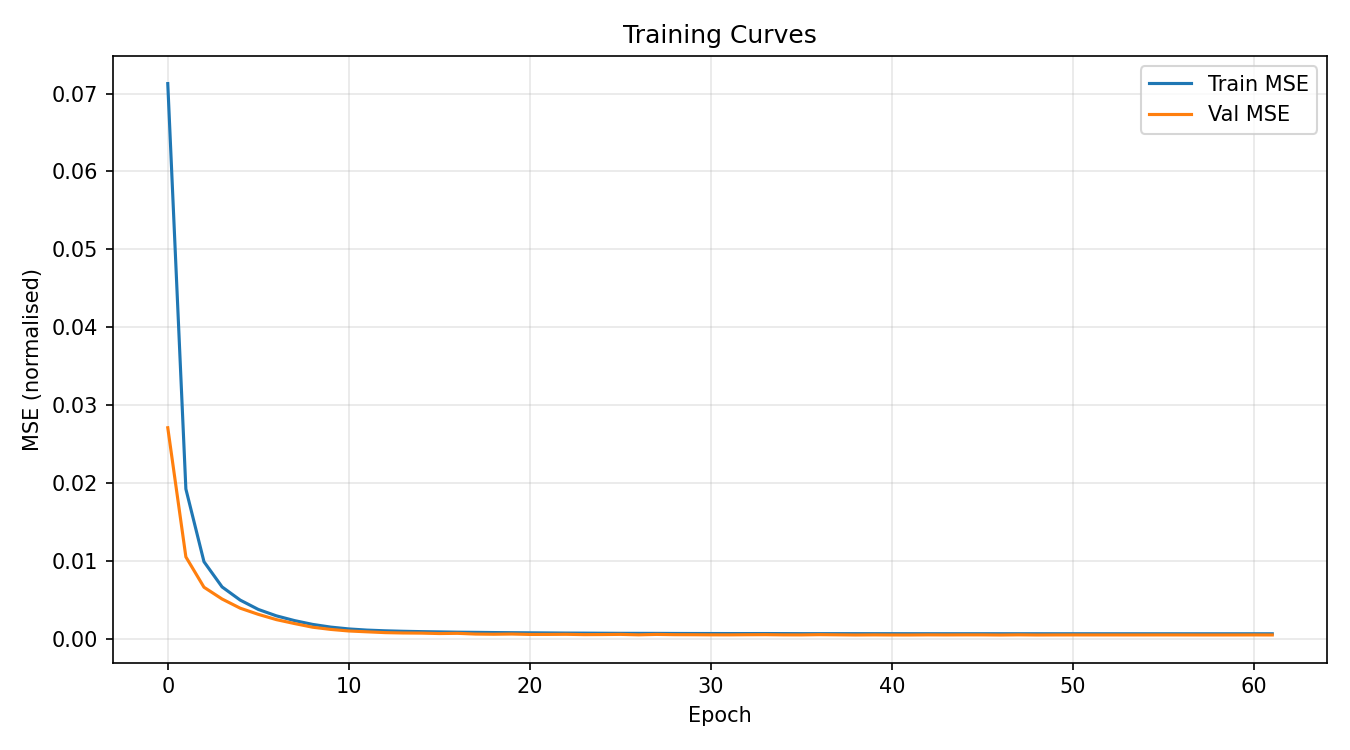
\includegraphics[width=0.8\textwidth]{Figures/training_curve.png}
\caption{Training and validation loss curves over 200 epochs showing convergence of the Edge MLP model with early stopping.}
\label{fig:training_curve}
\end{figure}

\section{Distance-Band Analysis}
\label{sec:distband}

The distribution of spatial errors was analyzed per band. In the 2.0--3.0 meter band, the range MAE was 0.116 meters, and the angular MAE was 6.66 degrees. In the 3.0--5.0 meter band, the range MAE was 0.119 meters, and the angular MAE was 3.62 degrees. As expected, range error remained consistent across bands indicating that the network is able to de-weight near-field multipath Wi-Fi. However, angular error decreased with increasing distances due to near-field lateral displacement resulting in greater angular sweeps relative to a fixed spatial resolution of the radar.

\begin{table}[htbp]
\centering
\caption{Error by distance band}
\label{tab:error_distance}
\begin{tabular}{lccc}
\toprule
\textbf{Band} & \textbf{N} & \textbf{MAE $r$} & \textbf{MAE $\theta$} \\
\midrule
2--3 m        & 566        & 0.116            & 6.66$^\circ$          \\
3--5 m        & 794        & 0.119            & 3.62$^\circ$          \\
\bottomrule
\end{tabular}
\end{table}

\section{Fused vs. Raw Comparison}
\label{sec:fusedraw}

As described above, capability comparisons among the modalities indicate that raw radar yields a range error of 0.15 to 0.65 meters, can handle angles, but will fail when there is no line-of-sight. Raw Wi-Fi yields a range error of 1.10 to 4.80 meters, cannot yield angles, but can provide obstruction handling. Finally, the fused ML model provides a range error of 0.118 meters, while also yielding both angles and obstruction handling capabilities. Radar occlusion demonstrates the ability of the system to perform low Euclidean errors during temporal reasoning using only forward filled Wi-Fi characteristics.

\begin{table}[htbp]
\centering
\caption{Sensor comparison}
\label{tab:sensor_comp}
\begin{tabular}{lccc}
\toprule
\textbf{Source} & \textbf{MAE $r$ (m)} & \textbf{Angle?} & \textbf{Walls?} \\
\midrule
Raw Radar       & $\pm$0.15--0.65      & Yes             & No              \\
Raw Wi-Fi FTM   & $\pm$1.1--4.8        & No              & Yes             \\
\textbf{ML Fusion} & \textbf{0.118}       & \textbf{Yes}    & \textbf{Yes}    \\
\bottomrule
\end{tabular}
\end{table}

\begin{table}[htbp]
\centering
\caption{Performance during occlusion}
\label{tab:perf_occlusion}
\begin{tabular}{lcc}
\toprule
\textbf{Condition} & \textbf{N} & \textbf{Euclid. MAE} \\
\midrule
Radar available    & 1,163      & 0.262 m              \\
Radar occluded     & 197        & 0.226 m              \\
\bottomrule
\end{tabular}
\end{table}

\section{Edge Inference Performance}
\label{sec:edgeinference}

Benchmarking performance of ESP32-S3 inference shows that the model is 11.6~KB in size with 2,474 float32 parameter values. It has an internal SRAM footprint of 32~KB. Inference latency is about 350 microseconds ($\mu$s) per window, or more than 99\% available processing headroom unused. We did not evaluate integer quantization as we determined that reducing the 6 meter measurement space to 256 bins would introduce a 2.35 centimeter (cm) root mean square (rms) noise floor that would be compounded by subsequent hidden layer operations. Given its size, the model will fit fully within internal memory and thus avoid latency associated with DRAM access.

\begin{table}[htbp]
\centering
\caption{ESP32-S3 inference benchmarks}
\label{tab:edge_inference}
\begin{tabular}{ll}
\toprule
\textbf{Metric} & \textbf{Value} \\
\midrule
Model file size   & 11.6 KB \\
Tensor arena      & 32 KB (internal SRAM) \\
Inference latency & $\sim$350 $\mu$s \\
Real-time budget  & 50,000 $\mu$s (50 ms) \\
Headroom          & \textbf{99.3\% unused} \\
Conversion loss   & $1.79 \times 10^{-7}$ \\
Framework         & TFLite Micro, Float32 \\
\bottomrule
\end{tabular}
\end{table}

\begin{figure}[htbp]
\centering
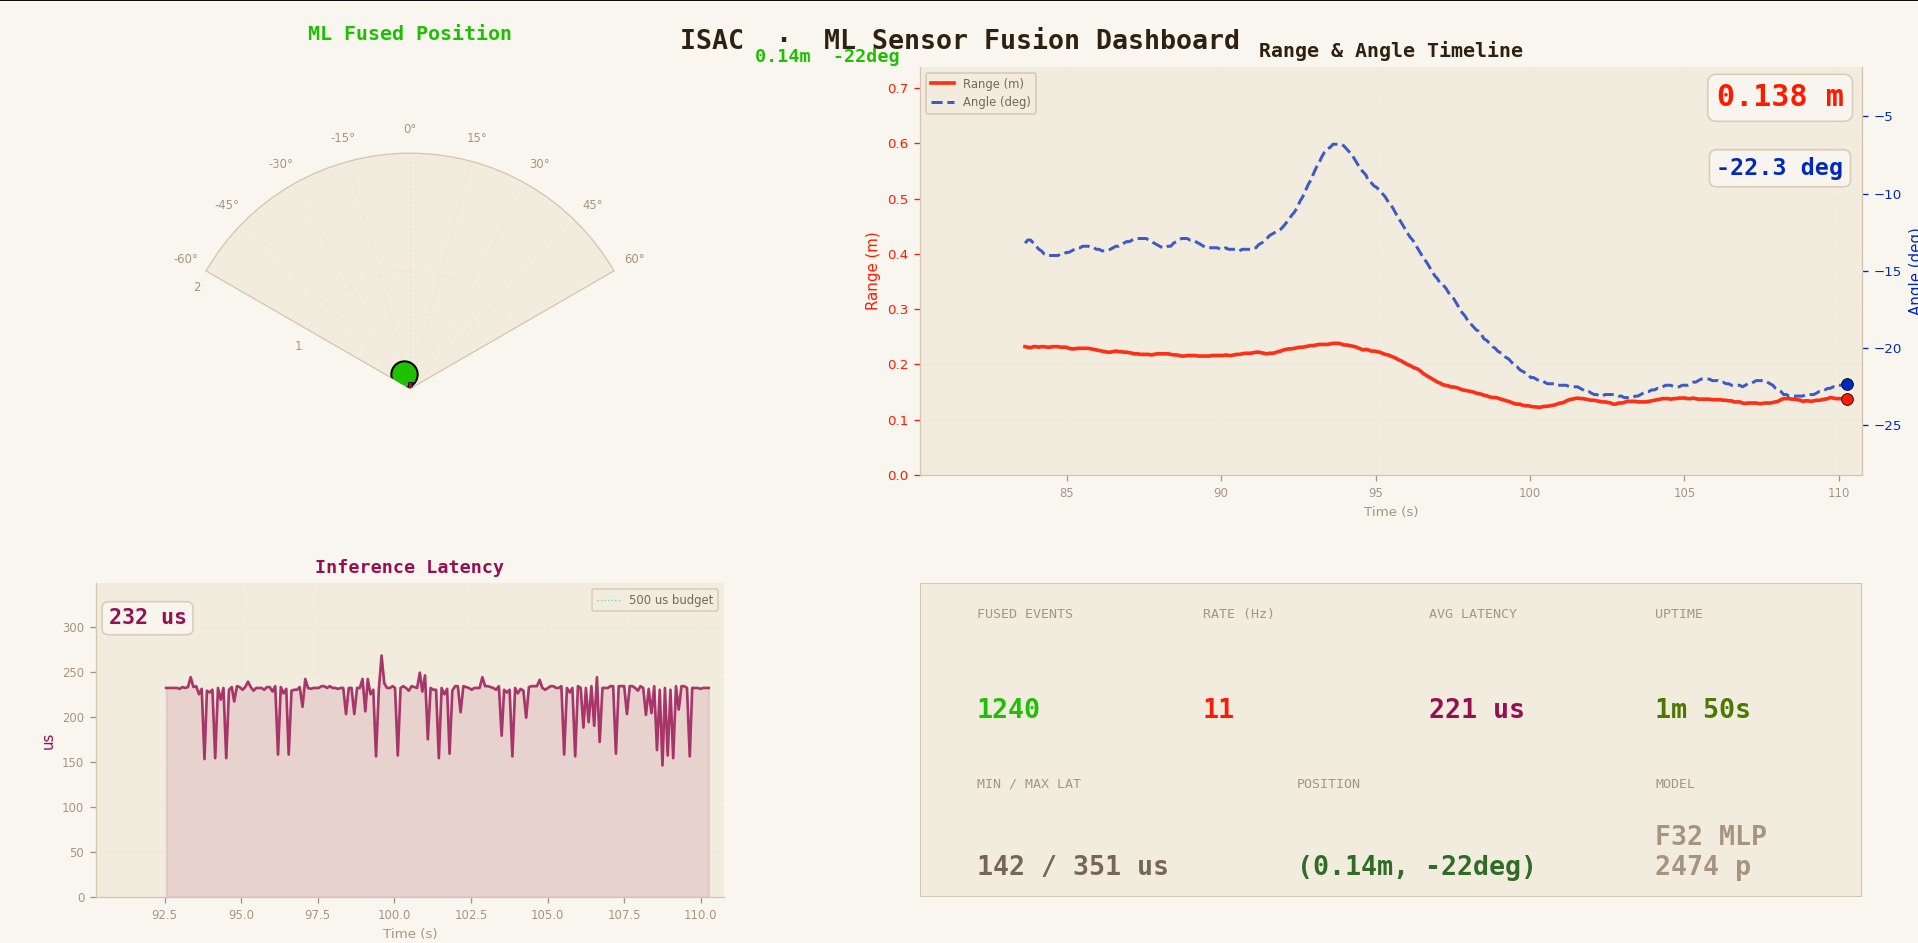
\includegraphics[width=0.9\textwidth]{Figures/Dashboard-fusedWithInferenceTimes.png}
\caption{Real-time dashboard showing fused position estimates with inference timing metrics on the ESP32-S3 platform.}
\label{fig:dashboard}
\end{figure}

\section{DCI vs. Machine Learning (ML)}
\label{sec:dcivsml}

DCI mathematically works based upon three variables at one time while the machine learning model uses twenty five variables allowing it to have far more temporal information. DCI also locks radar trust to its prior covariance, preventing it from adapting during the crossover region where Wi-Fi is superior to radar. Conversely, the machine learning model adapts based upon the magnitude of input features and their age flags. Additionally, DCI models velocity but does not do so effectively and does not model acceleration; conversely, the machine learning model implicitly models kinematic derivatives by utilizing the entire window of input features. Lastly, although there is no need for training data or computational steps involved in executing a DCI algorithm, they require full mathematical transparency and thus retain value for rapidly deploying systems.

\section{Failure Scenario Resilience}
\label{sec:failure}

The four adverse scenarios examined in this study included (a) Field of View Escape, where DCI will spike the radar variance to infinity as soon as the target escapes from the radar cone, at which time DCI is forced to transition into 1-D Wi-Fi based on range alone. (b) Tangential Walk: If there is no radial velocity, the system can no longer make predictions about Wi-Fi position. In these cases the system depends on continuous update of the radar's angle to estimate rotation. (c) Pillar Occlusion: Instantaneous loss of line of sight causes a penalty adjustment of Wi-Fi extrapolation with velocity projection to fill in the hole until the target comes back into line of sight. (d) Statue Mode: When all motion ceases, the radar filter drops the track. However, the tag continues to maintain Wi-Fi session by sending out heartbeats that preserve the identity of the target until motion resumes. Therefore, the results demonstrate that multi-modal heterogeneous fusion successfully mitigates the individual shortcomings of both modalities for indoor localization.

\begin{figure}[htbp]
\centering
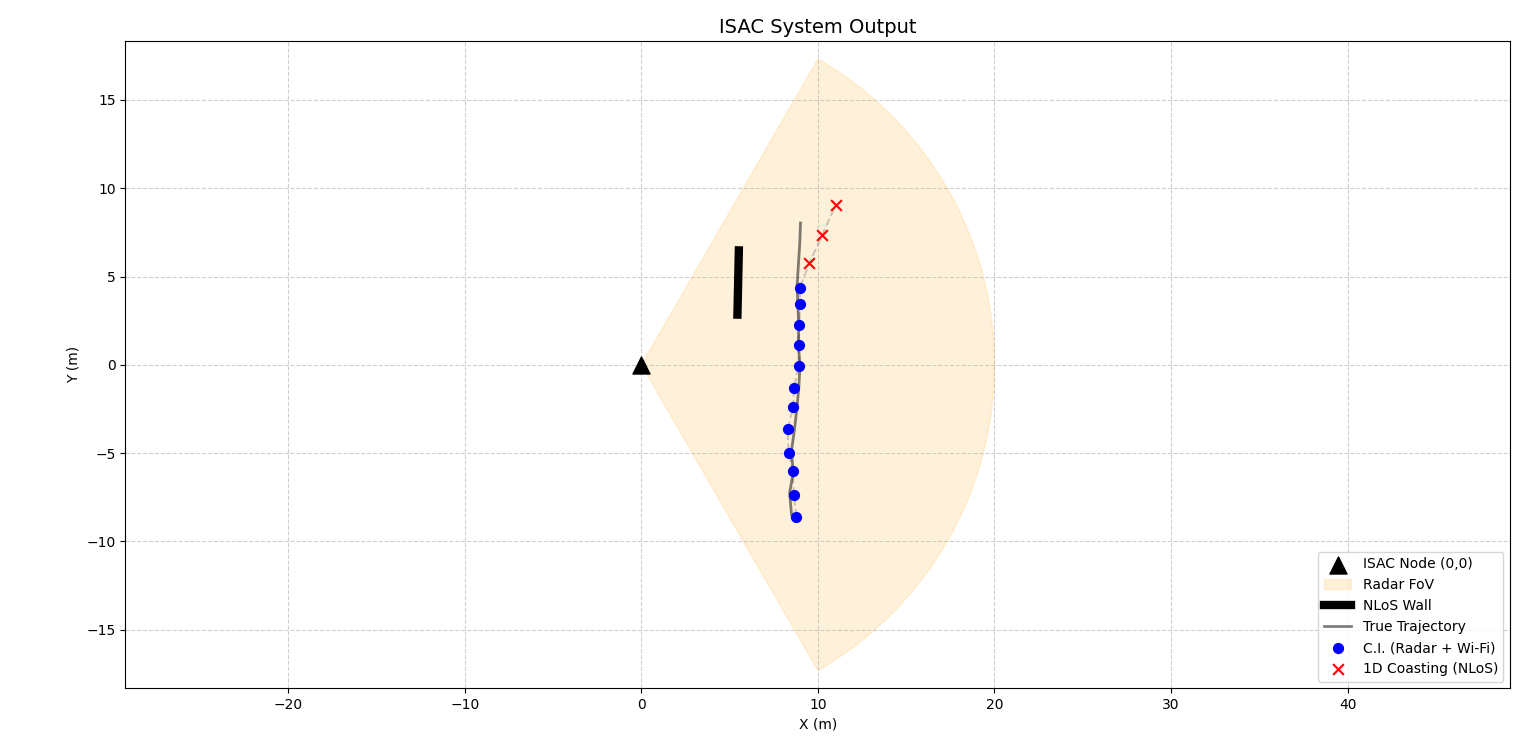
\includegraphics[width=0.9\textwidth]{Figures/PythonScenarioTestingSimulation.png}
\caption{Python test suite simulation results for the four failure scenarios: FOV escape, tangential walk, pillar occlusion, and statue mode.}
\label{fig:python_scenarios}
\end{figure}
